\documentclass[pdf]{beamer}

\mode<presentation>{
  \usetheme{Singapore}          % others: default Singapore Warsaw
  \usecolortheme{dolphin}       % beetle beaver orchid whale dolphin
  \setbeamertemplate{sections/subsections in toc}[ball unnumbered]  % others: circle ball square
	\usepackage{graphicx}
  \graphicspath{ {figures/} }
  \usepackage{listings}
  \lstset{
    basicstyle=\tiny\color{blue},
    frame=none,
    tabsize=2,
    showspaces=false,
    showtabs=false
  }
  \hypersetup{
    colorlinks=true,
    allcolors=blue
  }
}

% preamble
\title{How do Jinja2 filters work?}
\subtitle{a short introduction to ansible filters}
\author{Frank Jung}
\institute{frankhjung@linux.com}
\date{ \today }
\logo{ 
\includegraphics[height=1.5cm]{logos.png} }

\begin{document}

\begin{frame}
  \titlepage{}
\end{frame}

% \begin{frame}{Contents}
%   \tableofcontents{}
% \end{frame}

\begin{frame}
  \frametitle{Topics}
  What we will cover \ldots
  \pause{}
  \begin{itemize}
    \item what are Ansible filters?
      \pause{}
    \item when and where to use filters
      \pause{}
    \item when documentation is not enough
      \pause{}
    \item should I roll my own?
  \end{itemize}
\end{frame}

\section{What are Ansible Filters?}

\begin{frame}
  \frametitle{What are Ansible Filters?}
  Filters are from a fast, flexible, Python template engine called \ldots
  \pause{}
  \begin{center}
    \begin{figure}
      
\includegraphics[width=0.5\textwidth]{jinja.png}
    \end{figure}
    \href{http://jinja.pocoo.org}{jinja.pocoo.org}
  \end{center}
\end{frame}

\begin{frame}
  \frametitle{What are Ansible Filters?}
  Filters are used to transform data \ldots
  \pause{}
  \begin{enumerate}
    \item{they can be used inside a template expression}
      \pause{}
    \item{they can be used to manipulate local data}
  \end{enumerate}
\end{frame}

\begin{frame}
  \frametitle{What are Ansible Filters?}
  Some important features of filters \ldots
  \pause{}
  \begin{enumerate}
    \item{sand boxed}
      \pause{}
      \begin{itemize}
        \item{so can be used to evaluate untrusted code}
      \end{itemize}
      \pause{}
    \item{they are executed on the Ansible controller}
      \pause{}
      \begin{itemize}
        \item{\textcolor{red}{\textbf{not}} on the task's target host}
      \end{itemize}
      \pause{}
    \item{Ansible ships with its own filters}
      \pause{}
      \begin{itemize}
        \item{or use standard filters from Jinja2}
          \pause{}
        \item{or write your own!}
      \end{itemize}
  \end{enumerate}
\end{frame}

\section{Typical Use Cases}

\begin{frame}[fragile]
  \frametitle{Typical Filter Use Cases}
  \setbeamercolor{normal text}{fg=gray}
  \setbeamercolor{alerted text}{fg=blue}
  \usebeamercolor{normal text}
  Use filters to manipulate local data \ldots
  \begin{itemize}[<+->]
    \item \alert<1>{create new facts}
  \end{itemize}
  \begin{lstlisting}
  - name: count skills
    set_fact:
      skills_length: "{{ martin.skills | length }}"
  \end{lstlisting}
\end{frame}

\begin{frame}[fragile]
  \frametitle{Typical Filter Use Cases}
  \setbeamercolor{normal text}{fg=gray}
  \setbeamercolor{alerted text}{fg=blue}
  \usebeamercolor{normal text}
  Use filters to manipulate local data \ldots
  \begin{itemize}
    \item {create new facts}
    \item \alert<1>{subset or filter lists}
  \end{itemize}
  \begin{lstlisting}
  - debug:
      var: item
    with_items: "{{ martin.skills }}"
    when: item | match('p.*')

  - debug:
      var: item
    with_items: "{{ martin.skills }}"
    when: not item | match('perl') # same as item != 'perl'
  \end{lstlisting}
\end{frame}

\begin{frame}[fragile]
  \frametitle{Typical Filter Use Cases}
  \setbeamercolor{normal text}{fg=gray}
  \setbeamercolor{alerted text}{fg=blue}
  \usebeamercolor{normal text}
  Use filters to manipulate local data \ldots
  \begin{itemize}
    \item {create new facts}
    \item {subset or filter lists}
    \item \alert<1>{manipulate strings}
  \end{itemize}
  \begin{lstlisting}
  - debug:
      msg: "{{ martin.job | lower }}"

  - debug:
      var: item
    with_items: "{{ martin.name.split(' ') }}"

  - name: capitalize skills
    debug:
      msg: "{{ item | capitalize }}"
    with_items: "{{ martin.skills }}"
  \end{lstlisting}
\end{frame}

\section{Help}

\begin{frame}[fragile]
  \frametitle{Getting help when things go wrong}
  New in Ansible 2.3 is \verb type_debug :
  \begin{lstlisting}
  - debug:
    msg: "{{ martin | type_debug }}"
  \end{lstlisting}
\end{frame}

\begin{frame}[fragile]
  \frametitle{Getting help when things go wrong}
  Ansible Project - Google Groups
  \begin{center}
    \begin{figure}
      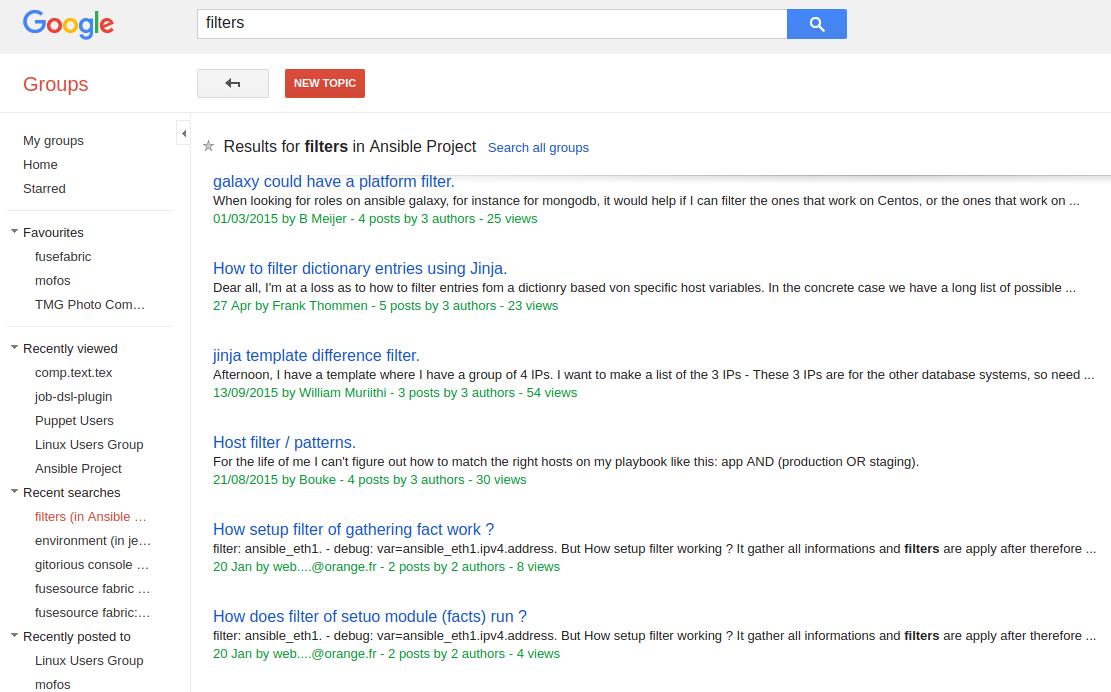
\includegraphics[width=0.8\textwidth]{ansible-google-group.png}
    \end{figure}
  \end{center}
  \tiny \url{https://groups.google.com/d/forum/ansible-project}
\end{frame}

\begin{frame}[fragile]
  \frametitle{Getting help when things go wrong}
  Read the source, for example Jinja has a sort method \ldots
  \newline
  \texttt{
    \tiny \url{https://github.com/pallets/jinja/blob/master/jinja2/filters.py}
  }
  \begin{lstlisting}
def do_sort(environment, value, reverse=False, case_sensitive=False, attribute=None):
    """Sort an iterable.  Per default it sorts ascending, if you pass it
    true as first argument it will reverse the sorting.
...
  \end{lstlisting}
  \pause{}
  \begin{lstlisting}
FILTERS = {
  'abs':                  abs,
  'attr':                 do_attr, 
...
  'sort':                 do_sort,
...
}
  \end{lstlisting}
  \pause{}
  Which gives a hint on how to use this method:
  \begin{lstlisting}
  - name: sort skills
    debug:
      var: item
    with_items: "{{ martin.skills | sort(reverse=True) }}"
  \end{lstlisting}
\end{frame}

\section{Roll Your Own}

\begin{frame}
  \frametitle{Writing your own filter}
  You may think to start here \ldots
  \begin{itemize}
    \item \small \url{http://docs.ansible.com/ansible/dev_guide/developing_plugins.html}
  \end{itemize}
  \pause{}
  But, that only redirects you to
  \href{https://github.com/ansible/ansible/blob/devel/lib/ansible/plugins/filter/core.py}{lib/ansible/plugins/filter} \ldots
\end{frame}

\begin{frame}
  \frametitle{Writing your own filter}
  Better, \href{https://opensolitude.com/2016/05/21/ansible-jinja2-filter-plugins.html}{Enhance your Ansible playbooks with custom Jinja2 filters}
  \begin{itemize}
    \item \small \url{https://opensolitude.com/2016/05/21/ansible-jinja2-filter-plugins.html}
  \end{itemize}
\end{frame}

\begin{frame}
  \frametitle{Writing your own filter}
  To create a custom filter the steps are simple \ldots
  \begin{itemize}
    \item write a test for your plugin
      \pause{}
    \item create a directory \texttt{filter\_plugins}
      \pause{}
    \item add a template file \texttt{collection.py} to this directory
      \pause{}
    \item define your method
      \pause{}
    \item add method to \texttt{FilterModule} class that implements \texttt{filters} method
      \pause{}
    \item re-test
  \end{itemize}
\end{frame}

\section{Summary}

\begin{frame}
  \frametitle{What we covered \ldots}
    \pause{}
  \begin{itemize}
    \item{what filters are}
      \pause{}
    \item{typical places you will use them}
      \pause{}
    \item{getting help when things go wrong}
      \pause{}
    \item{writing your own filter}
  \end{itemize}
\end{frame}

\begin{frame}
  \frametitle{References}
  \begin{itemize}
    \item
      \href{https://www.ansible.com/}{www.ansible.com}
      \begin{itemize}
        \item \href{http://docs.ansible.com/ansible/playbooks_filters.html}{filters}
        \item \href{https://github.com/ansible/ansible}{github}
      \end{itemize}
    \item
      \href{https://groups.google.com/d/forum/ansible-project}{Ansible Project - Google Groups}
    \item
      \href{https://opensolitude.com/2016/05/21/ansible-jinja2-filter-plugins.html}{Enhance your Ansible playbooks with custom Jinja2 filters}
    \item
      \href{http://jinja.pocoo.org/}{jinja.pocoo.org}
      \begin{itemize}
        \item \href{http://jinja.pocoo.org/docs/2.9/templates}{filters}
        \item \href{https://github.com/pallets/jinja}{github}
      \end{itemize}
  \end{itemize}
\end{frame}

\end{document}
